\documentclass{ufpatcc}

\include{include}
%% Packages used for the TCC

%\usepackage{booktabs}

%%%% Definitions and New commnads %%%%

\newcommand{\sen}{\operatorname{sen}}
\newcommand{\mbeq}{\overset{!}{=}}

\renewcommand\Re{\operatorname{Re}}
\renewcommand\Im{\operatorname{Im}}

%%%% New control sequences %%%%

\newcommand{\redeq}[1] {\textcolor{red}{#1}}
\newcommand{\blueeq}[1] {\textcolor{blue}{#1}}
\newcommand{\att}[1] {\textcolor{red}{#1}}
% Used Packages:
\usepackage{tikz}
\usepackage{float}
\usepackage{steinmetz}
\usetikzlibrary{arrows,shapes,shapes.multipart}
%\usepackage[brazil]{babel}
\usepackage[T1]{fontenc}
\usepackage[utf8]{inputenc}
\usepackage{amsmath}
\usepackage{amsfonts}
\usepackage{enumitem} % To adjust lists
\usepackage{verbatim} % Multi-line comments
\usepackage{mathabx} % Package that contains the circular convolution symbol
\usepackage{graphicx}
\usepackage{caption}
\usepackage{subcaption}
\usepackage{units}
\usepackage{adjustbox}
\usepackage{dirtytalk}

%\usepackage[backend=bibtex8]{biblatex}

\ifpdf

\ifdefined\hyperref
\else
\usepackage[pdftex,colorlinks]{hyperref}
\fi

\hypersetup{%
pdftitle={Some title},
pdfauthor={Your name - LaPS - UFPA},
pdfkeywords={DSP,Signal},
pdfstartview={FitH}, %% <--
urlcolor=black,
%linkcolor=blue,
linkcolor=black,
%citecolor=red,
citecolor=black,
}

% Ensiar o Latex a separar silabas
\hyphenation{DMT En-ge-nhei-ro}


\ufpaTitulo{An FPGA-Based Radion Frontend for LTE Transmission on Cloud RAN}

\ufpaAutor{Gabriel Peixoto de Carvalho}
\ufpaSegundoAutor{}
\ufpaOrientador{Prof. Aldebaro Barreto da Rocha Klautau Junior}
\ufpaCoordenadorCurso{Prof. Jos\'{e} Augusto de Lima Barreiros}

\ufpaCoOrientador{Prof. Wilson Pacheco Ferreira}
\ufpaMembroBancaA{Prof. Francisco Carlos Bentes Frey Muller}
\ufpaMembroBancaB{Eng. Igor Mesquita de Almeida}


\begin{document}

\ufpaPaginaDeRosto

\ufpaPagRostodo

\ufpaPaginaDeAprovacao

%%%%%%%%%%%%%%%%%%%%
%   Oferecimento   %
%%%%%%%%%%%%%%%%%%%%

\begin{ufpaOferecimento}
\index{Oferecimento@Oferecimento}%
\addcontentsline{toc}{chapter}{Dedicat�ria}

\end{ufpaOferecimento}

%%%%%%%%%%%%%%%%%%%%
%  Agradecimento   %
%%%%%%%%%%%%%%%%%%%%

\begin{ufpaAgradecimentos}
\index{Agradecimentos@Agradecimentos}
\addcontentsline{toc}{chapter}{Agradecimentos}

\begin{flushright}
Gabriel Peixoto de Carvalho
\end{flushright}

\end{ufpaAgradecimentos}

%%%%%%%%%%%%%%%%%%%%
%      Ep�grafe     %
%%%%%%%%%%%%%%%%%%%%

\begin{ufpaEpigrafe}
Viva como se voc� fosse morrer amanh�. Aprenda como se voc� fosse viver para sempre.\\
\begin{flushright}Mahatma Gandhi\end{flushright}
\end{ufpaEpigrafe}

%%%%%%%%%%%%%%%%%%%%%
%  Lista de Siglas  %
%%%%%%%%%%%%%%%%%%%%%

\chapter*{Lista de Siglas} \label{sec:siglas}
\begin{enumerate}
 \item ADSL - \textit{Linha de assinante digital assim�trica}
 %\item AWGN - \textit{Ru�do aditivo branco Gaussiano}
 %\item BER - \textit{Taxa de erro de bit}
 %\item DFT - \textit{Transformada de Fourier discreta}
 %\item DMT - \textit{Multi-tom discreto}
 %\item DSL - \textit{Linha de assinante digital}
 %\item FEQ - \textit{Equalizador em frequ�ncia}
 %\item FFT - \textit{Transformada rápida de Fourier}
 %\item FTTH - \textit{Fibra até a residência}
 %\item G.fast - \textit{Acesso rápido aos terminais do assinante}
 %\item ICI - \textit{Interferência inter-portadora}
 %\item IDFT - \textit{Transformada de Fourier discreta inversa}
 %\item IFFT - \textit{Transformada rápida de Fourier inversa}
 %\item ISI - \textit{Interferência inter-simbólica}
 %\item OFDM - \textit{Modulação por divisão ortogonal de frequência}
 %\item PC - \textit{Prefixo cíclico}
 %\item PSD - \textit{Densidade espectral de potência}
 %\item RIC - \textit{Resposta impulsiva do canal}
 %\item SC - \textit{Sufixo cíclico}
 %\item SER - \textit{Taxa de erro de símbolo}
 %\item SNR - \textit{Razão sinal ruído}
 %\item VDSL - \textit{Linha de assinante digital com taxa de bit muito alta}
 %\item 4GBB - \textit{Quarta geração de banda larga}
\end{enumerate}
 


\chapter*{Lista de S�mbolos} \label{sec:simbolos}
\begin{description}[labelsep=5em, align=left,labelindent=2cm]
\item[$b$] Taxa agregada de bits alcancavel para o sistema
%\item[$f_s$] Frequência de amostragem
%\item[$H(f)$] Espectro do canal
%\item[$H_k$] Ganho do $k$-ésimo subcanal
%\item[$\mathbf{ H_\text{ICI}}$] Matriz de ICI no domínio do tempo
%\item[$\mathbf{ H_\text{ISI}}$] Matriz de ISI no domínio do tempo
%\item[$L$] Dispersão do canal
%\item[$n$] Índice da amostra
%\item[$n_0$] Indice da amostra de início do símbolo recebido para o receptor sincronizado
%\item[$N$] Número de pontos da DFT ou tamanho do vetor símbolo DMT
%\item[$N_a$] Número de amostras afetadas por ISI e ICI
%\item[$p_k$] Parte real do $k$-ésimo subsímbolo
%\item[$P_x$] Potência total de transmissão
%\item[$q_k$] Parte imaginária do $k$-ésimo subsímbolo
%\item[$\mathbf{Q}$] Matriz DFT
\end{description}


%%%%%%%%%%%%%%%%%%%%%%%%%%%%%%%%%%%%%%%%%%%%
%  Insere a lista de Figuras e de Tabelas  %
%%%%%%%%%%%%%%%%%%%%%%%%%%%%%%%%%%%%%%%%%%%%

\listoffigures \clearpage \listoftables \clearpage

%%%%%%%%%%%%%%%%%%%%
%      Sum�rio     %
%%%%%%%%%%%%%%%%%%%%

\tableofcontents    \clearpage

%%%%%%%%%%%%%%%%%%%%
%      Resumo      %
%%%%%%%%%%%%%%%%%%%%

\begin{ufpaResumo}


\end{ufpaResumo}

\begin{abstract}
    
The evolution of mobile services in terms of access technologies and application 
layers is driving a huge change in mobile communication systems. A recent hot 
topic in the field is the rise of the cloud computing paradigm, thus the idea 
known as cloud radio access networks (Cloud-RAN) is growing in the industry. 
This behavior comes from the potential of cloudification for improvement in the 
efficiency of resource allocation, manageability and power consumption, aspects 
inherent of traditional RANs.\\

Thus, with the emerging of C-RAN, several questions about how to implement and 
which tools to use come naturally. This work aims to evaluate the potential of a 
programmable fronthaul radio interface, as known, actual network does not have 
the adaptative capability needed for the C-RAN. For this work a setup of a radio 
unit, composed by two fpgas (one acting as the Baseband unit and other as the
(digital front-end) of the radio unity) connected through ethernet and two 
transceivers (analog front-end), one in each FPGA. Within this setup various 
algorithms can be tested and can be evaluated in LTE scenarios because the 
transceiver works in LTE and C-RAN .\\

This work shall focus on the evaluation of the radio interface and perform the 
tests inherent to it, exploring FPGA adaptability and parallelism with the 
internal and external communication protocols, and so exploring the advantages 
of the transceiver used, the fmcomms2  development board (AD9361 chip) from 
Analog devices, which is a device broadly used in software defined radio 
hardwares, as known as USRPs (Universal Software Radio Peripheral). \\

An aspect of the transceiver that is very attractive to the C-RAN paradigm is 
its configurability and scalability, capable of real-time adjustments in the 
sampling frequency or operation mode from 2x2 to 4x4 MIMO (Multiple Inputs and 
Multiple Outputs), this real-time adaptive characteristic is ideal to C-RAN 
environment.\\

The results are generated primarily aiming a fidelity in the transmitted and 
receiver signals, after these results are conclusive it is possible to proceed 
to more complex tests and approaches of this setup. Another test made was the 
analysis of the synchronization between  receiver and transceiver using a CIPRI 
emulator implemented in FPGA logic, which is the standard fronthaul interface, 
in this test it is possible to observe the advantages of the programmable radio 
front-end in the system.\\



\end{abstract}

%%%%%%%%%%%%%%%%%%%%%
%   Corpo do TCC    %
%%%%%%%%%%%%%%%%%%%%%

\pagenumbering{arabic}

\part{Introduction}
\chapter{Introduction}
\label{chap:intro}

%The world is much more interconnected and the economy is growing wilder and
%wilder, a lot of economical issues rise in different countries almost every
%year. The climate changes are also a concern to the modern governments, thus the
%idea of re-utilizing resources and  make these resources be more economically
%and environmentally friendly are a goal for modern research and development.

The scalability and reconfigurability of telecommunication systems is very
interesting for the companies and operators in the current economic needs,
re-utilization is the key to decrease deployment and equipment update. This work
aims to evaluate the feasibility of a radio-fronthaul System for
\textit{Long-Term Evolution} (LTE) transmissions in a reconfigurable and scalable
environment of \textit{Cloud Radio Access Network} (CRAN).

Cloud computing is a paradigm which use is getting more common in companies and
developers, it solves some infrastructure problems of small and big companies.
Companies do not need to own computers or anything locally to operate,
everything can be done remotely and a more experienced company and staff can
offer such infrastructure or application as a service. Such idea of having
everything as a service is very attractive both economically  and
environmentally because there is no waste of resource, everything is scalable to
the need of the client and upgradeable if needed.

The Radio access technologies have been evolving from audio traffic to intensive
data traffic over the recent standards, because the mobile devices got a myriad
of functions which could only be executed by \textit{Personal Computers} (PC).
Such networks demand a huge amount of resources. Hence, there are concerns about
how to develop and deploy these networks such as backwards compatibility of the
devices, because an operator would never deploy a network which is not
compatible with previous standards equipments, this is not profitable. Having
these ideas in mind the C-RAN concept began to be developed,  where the
resources for the RANs are scalable and configurable to needs of the clients and
operators, and where the baseband processing is all done on the cloud and the
radio frontends are reconfigurable to handle different data and modulation
outputs.

The reconfigurable fabric of the \textit{Field Programmable Gate Array} (FPGA)
technology is very attractive to implement such radio front-ends and other
reconfigurable computing tasks, because it is flexible to be reconfigured
on-the-run, offers a really good parallel processing and I/O capabilities. Thus
this work aims to evaluate the implementation feasibility of a radio frontend
LTE transmissions in a Cloud RAN environment (adaptability and
reconfigurability).

This work is implemented in a Xilinx Virtex 7 FPGA and using the transceiver
board \textit{FMCOMMS2} from \textit{Analog Devices}, this transceiver can be
reconfigured in real time and runs up to 6 GHz band, it has been chosen because
of such reconfigurability properties.

The remainder of this text is organized in 4 parts as follows:

Part II is a literature review of some theoretical background used in this work
development, divided in three chapters. Chapter \ref{chap:sdr} offers an
overview of Cloud and Software defined radio, because reconfigurability and
scalability are features desired in SDR field and in this work. In Chapter
\ref{chap:lte} there is an overview in Digital Communication Systems and LTE,
since this work shall focus on LTE  frequency band transmissions.

Part III is the core of the work, Chapter \ref{chap:implementation} describes
the implementation of this work's setup and gives an overview of functionalities
of both FPGA and Fmcomms2 shall be explained. The development will be described
in terms of how it was implemented in both FPGA logic and software drivers.

Part IV reports all the results of this work in Chapter
\ref{chap:results}. The configuration results report how the transceiver board
communication and configuration were done. The simulation results aim to show
the VHDL blocks simulation prior to hardware implementation and at last the
transmission results aim in report the integrity of the transmitted signals.

Part V presents the conclusions and future works in Chapter
\ref{chap:conclusion}, which aim to report everything learned from this work and
what can be done to improve the transmission/reception quality.

\part{Literature Review}
\chapter{Synchornization}

\section{Carrier Recovery}

Carrier recovery is a process used in coherent demodulation where the phase
and the frequency of the transmitter carrier wave are recovered by the receiver
and thus after having such information it is possible to extract the information
in the transmitted signal.\\
Considering that the phase and frequency of the transmitted wave probably will
be affected by noise, it is not a straight-forward method, it includes filtering
and usually feedback systems to correct the erros in phase or frequency caused
by the noise.\\
This chapter aims in the brief exploration of some techniques used for carrier
recovering, such as Phase locked loops, costas loop and others.\\

\subsection{Costas Loop}

\part{Implementation}
\chapter{Setup Description}


\section{Overview}

\section{Integration between FPGA and FMComms2}

\part{Final Results}
\chapter{Results}

\section{Preliminary Tests}

\section{Transmission Tests}


\part{Conclusion and Future Work}
\chapter{Conclusion}
\label{chap:conclusion}

\section{Conclusion}
\label{sec:conclusion}

The development of this setup was meant to be general and be used in both
research and academic environments. The process of implementing this setup went
through a myriad of fields in telecommunications and embedded systems, such as
communication protocols, embedded programming, electronics and many others,
being this setup a testbed for more complex processes inside the LTE band saves
a lot of time in development. \\

The FMComms2 board allows real-time and scalable change in parameters by
software or hardware signals, and it re-calibrates and reconfigures itself if
needed so, which makes a very good transceiver board to be used in a C-RAN
environment.\\

This setup was extensively documented and can be used in digital communication
classes to show how a real radio frontend system is made, of course there is
much to improve, there is no dynamic clock synchronization between the FPGA and
the FMComms2, there is no communication protocol between the FPGA (BBP) and the
external world other than the FMComms2 such things are necessary to have a real
frontend but were outside the scope of this project which was just to evaluate a
setup for a scalable and dynamically configurable frontend.\\

Although the FMComms2 and the FPGA operates on different clocks, thus no real
synchronization was implemented, this setup has the minimal capability of
transmitting and receiving signals and reconfigure itself on real-time, the main
goal of this work was reached, however there is much to explore with these tools
and devices.

\section{Future Works}
\label{sec:futurew}

Having finished this part of the work a natural sequel would be implementing
Ethernet connection driver in the FPGA, making it possible to receive data from
Ethernet and hand this to the transceiver board following the schematic on
figure \ref{fig:setupeth} idea. This would be a challenge because there is a lot
of things to consider, but the most problematic of them all is synchronization,
the clock in which everything inside the FPGA works is different from the AD9361
clock not only in frequency but in phase, this can bring a lot of problems,
however there is the possibility of feeding FMComms2 with an external clock
which would increase its performance.\\

With Ethernet it would be possible to generate the modulated samples and send
them trough air, just like Gnuradio + USRP and thus demodulate the received back
samples in the PC, however there is another possibility, modulation and
demodulation blocks implemented in the FPGA logic, thus much faster than the PC
ones and with partial reconfiguration there is the advantage of loading various
schemes of modulation/demodulation in the FPGA, implementing thus a very good
SDR. The Ethernet connection, is also very interesting for C-RAN
environment, because Ethernet is cheap and easy to implement.\\

\begin{figure}[htbp]
    \centering
    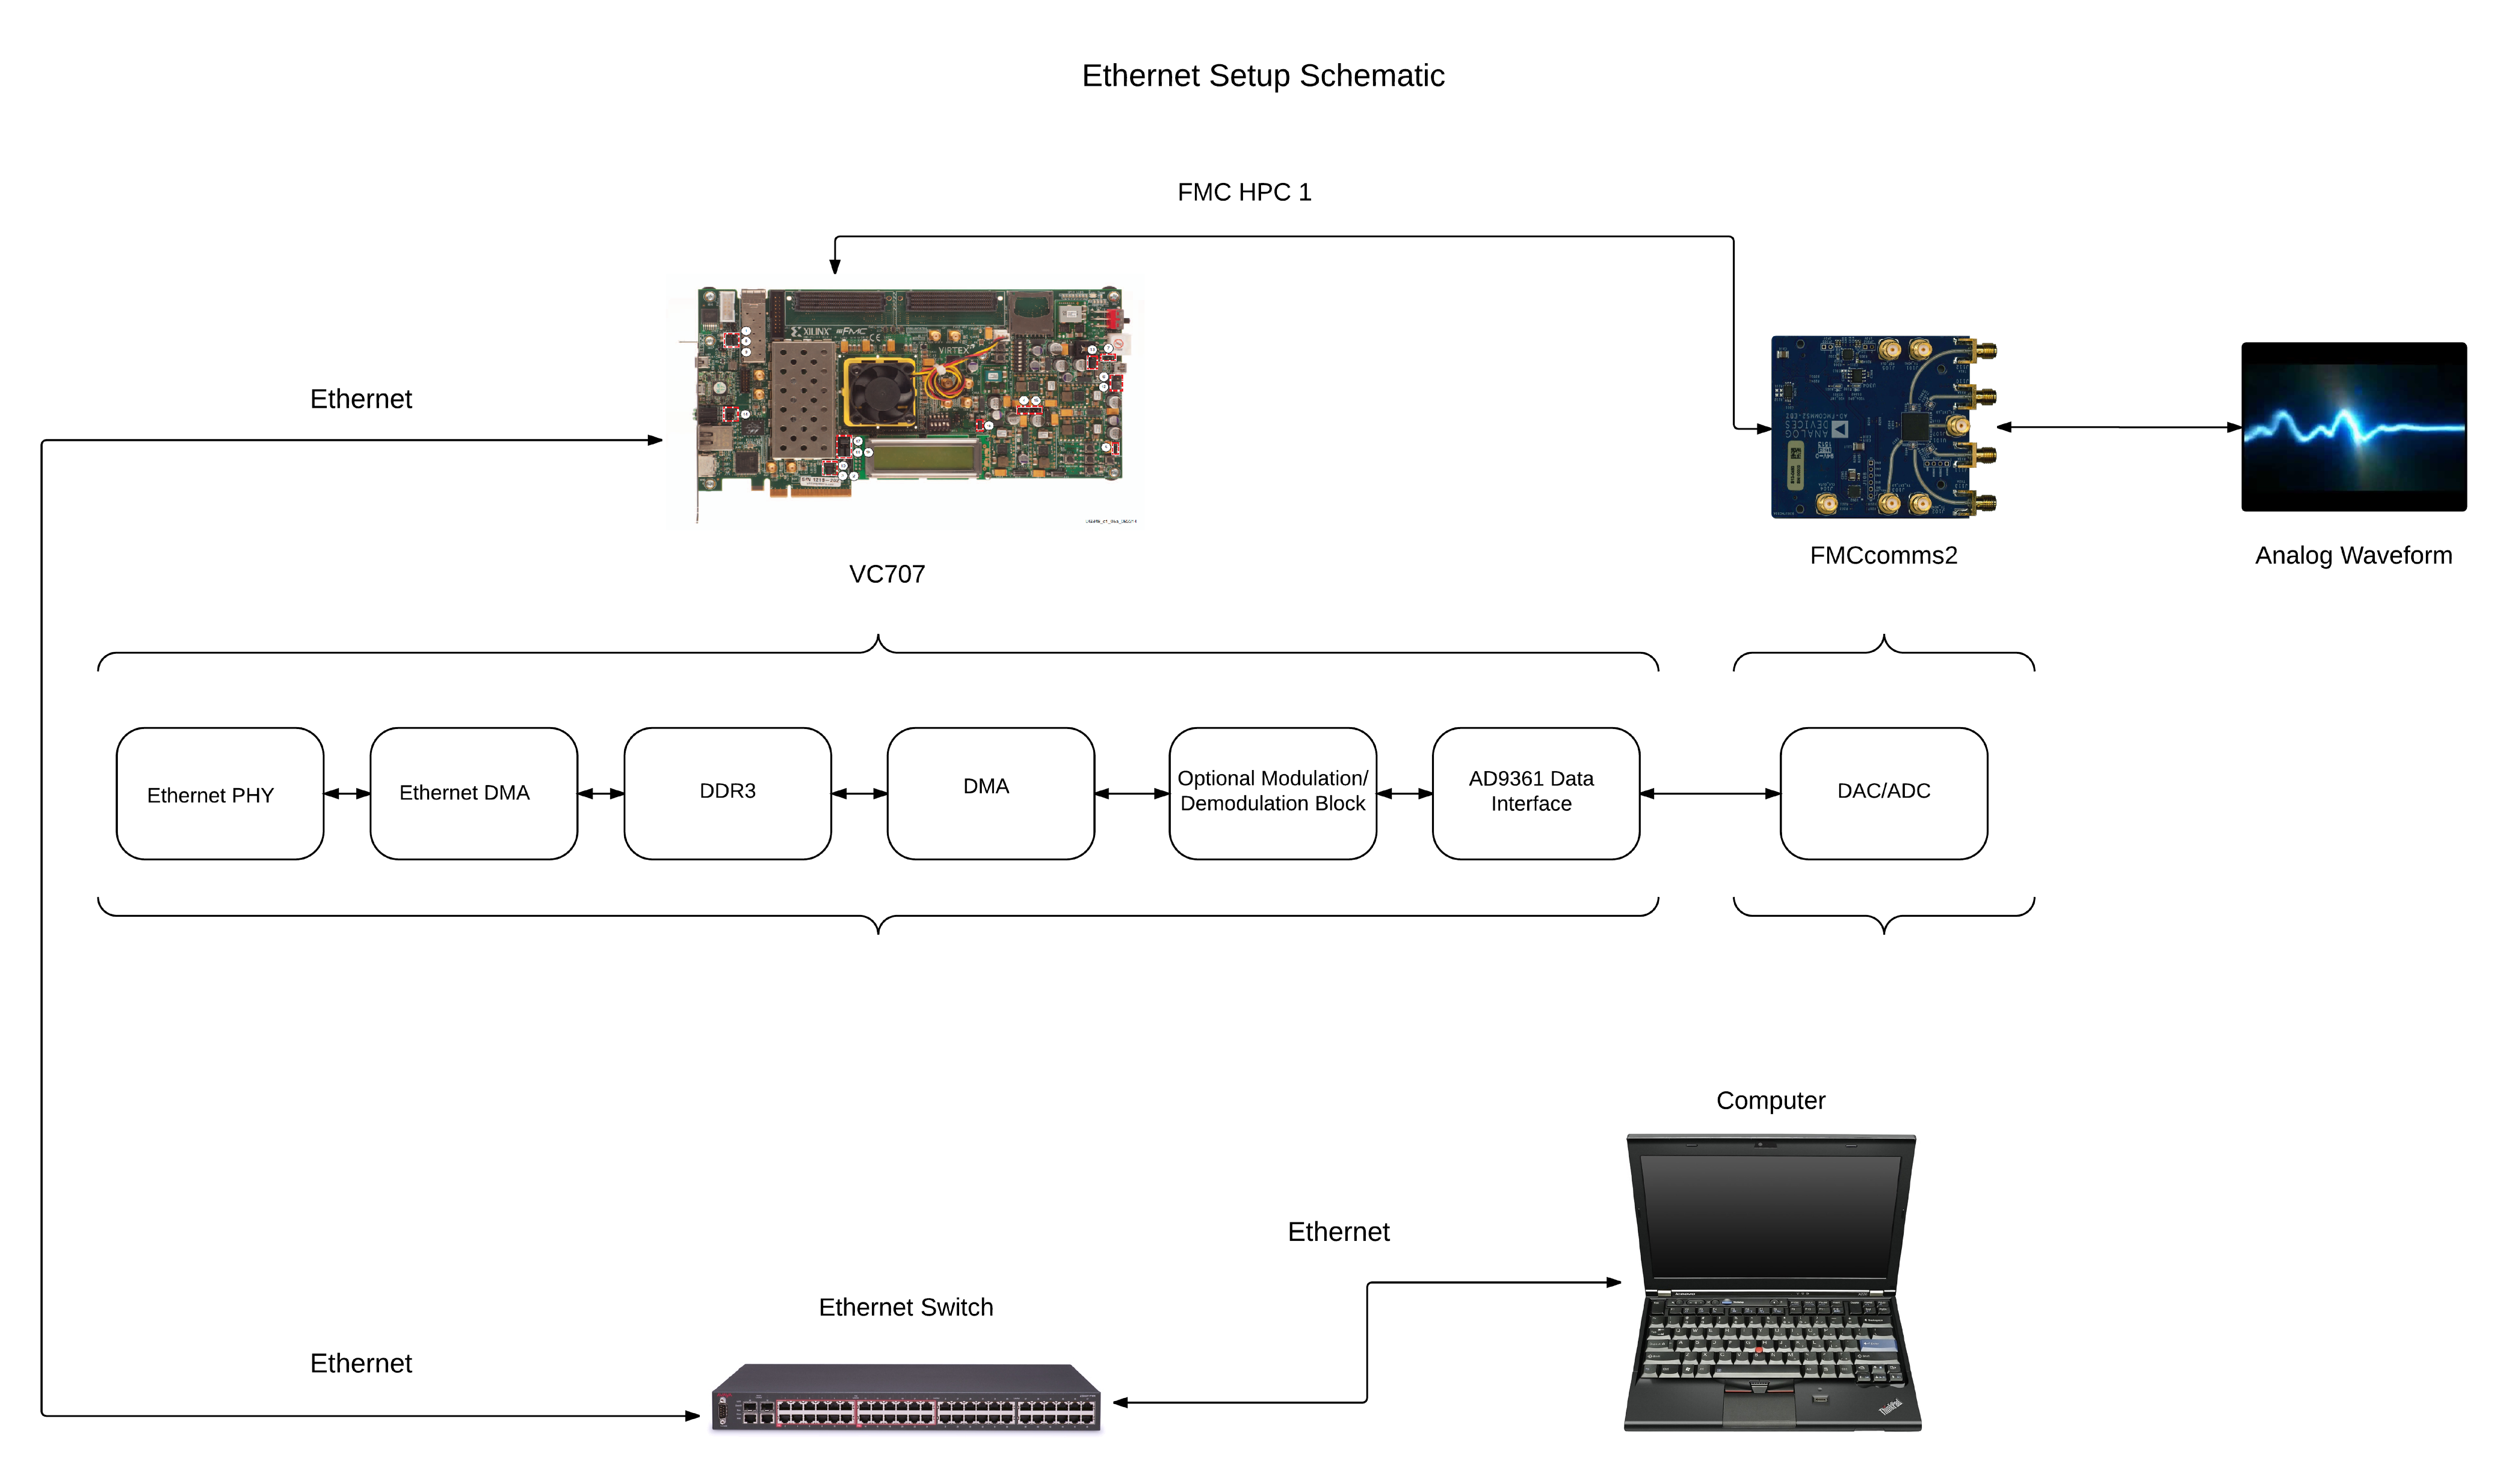
\includegraphics[width=0.65\textwidth]{./figures/eth_setup}
    \caption{ Setup Enhanced with Ethernet Connection
    \label{fig:setupeth}}
\end{figure}


%%%%%%%%%%%%%%%%%%%%%%%%%%%%%%%%%%`
%   Referencias bibliograficas   %
%%%%%%%%%%%%%%%%%%%%%%%%%%%%%%%%%%

\renewcommand\bibname{Refer�ncias Bibliogr�ficas}
%\bibliographystyle{../../../public/ABNT-20020112}
%\bibliographystyle{../public/IEEEtran}
%\bibliographystyle{../../../Public/IEEEtran_pt}
\bibliographystyle{abnt}
\bibliography{references}

%temorary tag just while there is no \citation
%eliminates no \citation error
\nocite{*}

\clearpage

%%%%%%%%%%%%%%%%%%%%%
%   Apêndices    %
%%%%%%%%%%%%%%%%%%%%%

\appendix
\chapter{PLL}
\chapter{FPGA Design Flow}
\chapter{AD9361 NO-OS Driver}


%%%%%%%%%%%%%%%%%%%%%
%   Página em branco    %
%%%%%%%%%%%%%%%%%%%%%

\newpage
\thispagestyle{empty}
\mbox{}

%% -- Termino do TCC
\end{document}
